\section{Análisis Bivariado}

\newcommand{\varnorm}[1] {
    (#1_t - \mu_{#1})
}

\newcommand{\squarederr}[1]{
    \sum\limits_{t=1}^n \varnorm{#1}^2
}

\newcommand{\crosscorr}[2]{
  \frac{\sum\limits_{t=|k|+1}^n \varnorm{#1} (#2_{t-k} - \mu_{#2})}{
    \sqrt{\squarederr{#1} \squarederr{#2}}
  } \\
}

\newcommand{\corrdenom}[2]{\sqrt{\squarederr{#1} \squarederr{#2}}}

En \cite{KOU2008.2} se continúa el trabajo en series de tiempo, y se efectúan análisis tanto por cada serie por separado como para las dos en conjunto, lo cual se llama ``Análisis bivariado'' en la terminología de series de tiempo.

Una posible medida del \entrainment se podría dar midiendo cuánto influye una serie sobre otra; este \entrainment sería direccional: queremos medir cuánto influye el interlocutor $A$ al interlocutor $B$ y viceversa. Puede darse el caso en que ambos tengan fuerte interacción, en tal caso hablamos de \emph{feedback}. En \cite{gravano2015backward} este concepto es definido como \emph{forward influence}.

\nota{Agustín, chequea si ésto que puse está bien}

Para medir cuánto se mimetizan las dos series, utilizaremos la función de correlación cruzada (c.c.f)\cite{CHATFIELD}, que mide cuánto se parecen la serie $X$ e $Y$ aplicando un desplazamiento $k$, dándonos un valor entre $-1$ y $1$ (similar a la correlación de la estadística clásica). Podemos aproximar la c.c.f. mediante la fórmula de la correlación cruzada muestral.

\begin{equation}
  r_{AB}(k) =
  \left\{
    \begin{array}{ll}
      \frac{\sum\limits_{t=|k|+1}^n \varnorm{A} (B_{t-k} - \mu_{B})}{\corrdenom{A}[B]} \\ & \mbox{si } k \geq 0 \\
      \crosscorr{B}{A} & \mbox{si } k < 0
    \end{array}
  \right.
\end{equation}

Podemos ver que, si $k \geq 0$, lo que hacemos es, a grandes rasgos, calcular la correlación de Pearson entre $A_{t+k}$ e $B_t$. Si $k < 0$, lo hacemos entre $A_t$ e $B_{t+k}$. Viéndolo de otra forma, si $k \geq 0$, estamos midiendo cuánto influye $B$ sobre $A$ contemplando un desplazamiento de $k$ puntos; si $k \leq 0$ medimos la influencia de $A$ sobre $B$ a misma distancia.


Para cada conversación, se grafica entonces el correlograma cruzado, considerando lags tanto positivos como negativos. En \ref{time_plot_with_bivariate} tenemos un gráfico de los time-plots de dos series de tiempo generadas de una conversación, junto a sus autocorrelogramas (ver \ref{sec:time_series}) y sus correlogramas cruzados

\nota{Kousidis menciona algo acerca de los problemas que se dan cuando hay feedback...¿qué deberíamos considerar al respecto de ésto?}

\nota{Mandar todo ésto a nuestra definición de TAMA}
\begin{align}
  A \rightarrow B &= max \{ r_{AB}(k), k \leq 0 \} \\
  B \rightarrow A &= max \{ r_{AB}(k), k \geq 0 \} \\
\end{align}


$A \rightarrow B$ es el entrainment direccional de $A$ hacia $B$, que mide cuánto se mimetiza $B$ a $A$. (explicar un poco más ésto)

\begin{figure}
\centering
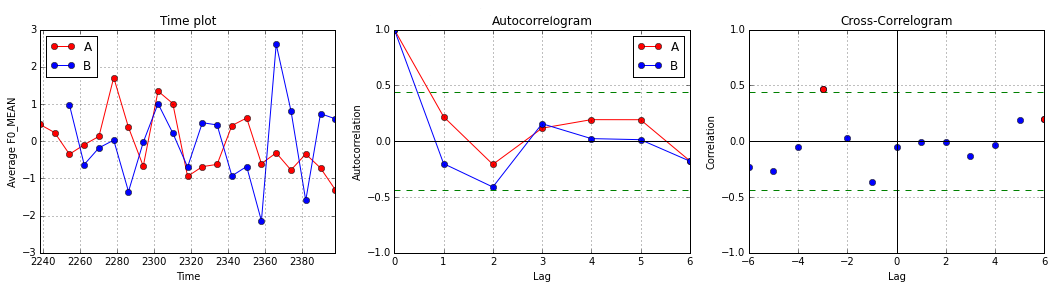
\includegraphics[width=15cm]{images/time_plot_with_cross_correlation.png}
\caption{Time-plot producido por TAMA, junto a su autocorrelación y correlación cruzada\label{time_plot_with_bivariate}}
\end{figure}
